% !Mode:: "TeX:UTF-8"
\chapter{H.265 帧内无损编码及优化算法硬件实现}
\label{cha:c4}
在视频实时编码的场景中,使用专用集成电路 (Application Specific Integrated Circuit, ASIC) 实现可做到功耗与性能的良好平衡,是业界的主流做法。本章介绍 H.265 帧内无损编码的 ASIC 实现,并给出行为级仿真结果。

\section{硬件系统框架}
如图 \ref{fig:HardwareArch} 所示,H.265 帧内无损编码器包含的主要模块有:帧内预测模块(分为 2 个阶段进行)、熵编码模块、环路后处理模块、变换量化模块(无损编码时跳过处理)以及与外部存储器交互的 Fetch 与像素 Buffer 模块,同时存在大量用于待编码系数的中间缓存模块,不一一列出。
\begin{figure}[hbt]
    \centering
    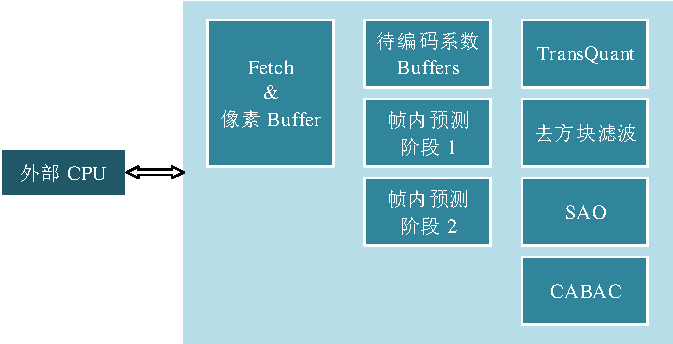
\includegraphics{HardwareArch.pdf}
    \caption{H.265 编码器硬件系统框架}
    \label{fig:HardwareArch}
\end{figure}

图中的外部 CPU 并非系统框架内的模块,系统框架预留了与外部控制器的交互接口,用于进行诸如感兴趣区域 (Range of Interest, ROI)、码率控制、时延控制等外部控制操作。

\section{关键模块的硬件实现}

根据前文所述,H.265 标准下在进行帧内预测时,需要对一个 PU 内的 35 种预测模式进行扫描,从而判断哪种模式是最优的。然而在硬件实现中出现一个问题:在进行预测之前,需要获取其经过重建的参考像素,而参考像素大概率位于前一个 PU 之中,因此,为了等待重建需要让整个预测处理在时序中长时间停留,导致系统吞吐率和硬件的利用率降低\upcite{FuDanIntraArchitecture},如图 \ref{fig:Intra12}(a) 所示。这一情况在处理大尺寸预测单元时尤为明显。
\begin{figure}[hbt]
    \centering
    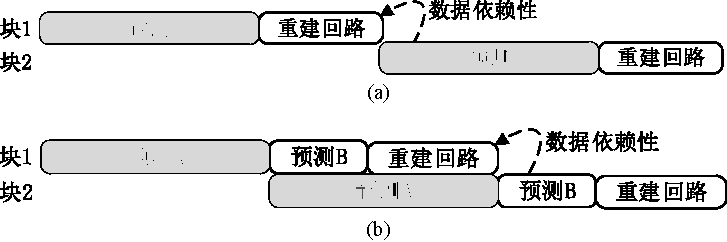
\includegraphics{Intra12.pdf}
    \caption{帧内预测时序说明}
    \label{fig:Intra12}
\end{figure}
基于上述分析,使用了如图 \ref{fig:Intra12}(b) 所示的硬件架构,将预测流程拆分为 2 部分进行:预测 A 使用原始像素而非重建像素作为参考点,来扫描所有的预测模式找出最优的一种,预测 B 与传统预测一致,使用重建像素作为参考点进行预测,但不进行扫描而是使用预测 A 找到的最佳模式直接计算结果,后续的残差计算、熵编码也是以预测 B 的输出结果为准进行的。尽管预测 A 得到的最佳模式可能与标准结果存在出入,但经过大量测试证明该影响可忽略不计,容忍这极少量的编码效率损失可换来更加流畅的系统流水线和更高的吞吐率,显然是值得的。最终该帧内预测模块的顶层结构如图 \ref{fig:Intra12Top} 所示。
\begin{figure}[hbt]
    \centering
    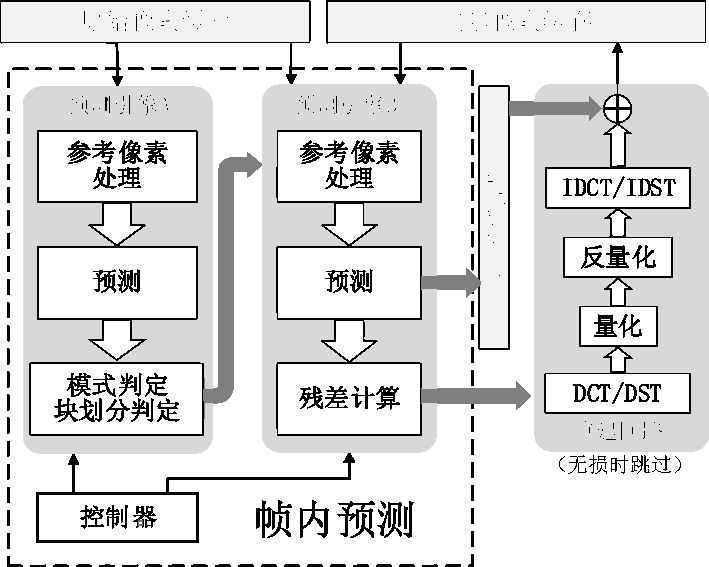
\includegraphics{Intra12Top.pdf}
    \caption{帧内预测模块顶层视图}
    \label{fig:Intra12Top}
\end{figure}

\section{行为级仿真与测试}
对所设计编码器进行行为级仿真,以验证其正确性。系统验证方案如图 \ref{fig:behavesim} 所示。
\begin{figure}[hbt]
    \centering
    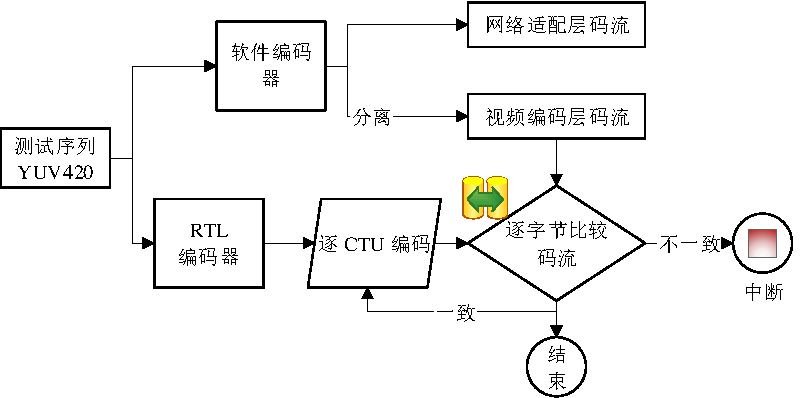
\includegraphics{behavesim.pdf}
    \caption{硬件编码器行为级仿真方案}
    \label{fig:behavesim}
\end{figure}
准备一已降采样为 YUV4:2:0 的测试视频序列,提前使用标准软件编码器进行编码,由于 H.265 标准中还规定了网络适配层码流的语法语义,而硬件编码器仅输出视频编码层码流,因此需要编写脚本抽取出软件结果的视频编码层码流作为对照数据。运行硬件编码器的行为级仿真,将其配置成与软件编码时的参数完全一致的状态,逐 CTU 编码测试序列,同时将编码结果的码流逐字节与对照数据进行比较,一旦出现不一致的情况即中断仿真流程。

行为级仿真在 Synopsys VCS 软件平台进行,同时使用 perl、make 等脚本进行辅助验证,实现全自动的行为级仿真验证。仿真结果如图 \ref{fig:behavesimScreen} 所示。
\begin{figure}[hbt]
    \centering
    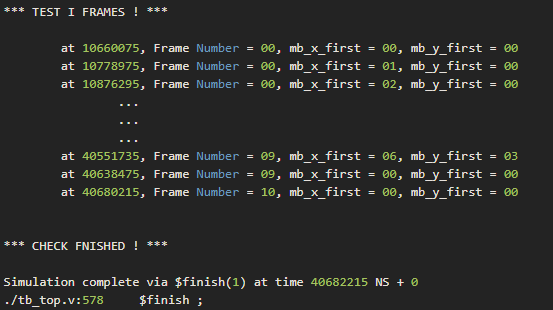
\includegraphics[scale=0.5]{behavesimScreen.png}
    \caption{硬件编码器行为级仿真屏幕截图}
    \label{fig:behavesimScreen}
\end{figure}

最后统计应用前文所述联合优化算法前后的行为级仿真编码结果,比较其编码所用时钟数及输出码流字节数。由于硬件行为级仿真耗时较长,仅统计 ClassA\textasciitilde ClassF 6 类测试序列中各一个序列的仿真结果,如表 \ref{tab:behavesimTab} 所示。
\begin{table}[hbt]
    \centering
    \caption{H.265 硬件编码器优化算法行为级仿真性能统计}
    \label{tab:behavesimTab}
    \begin{tabular}{@{}clcc@{}}
        \toprule
        序列类别                           & \multicolumn{1}{c}{序列} & 码率     & 编码时间(时钟数) \\ \midrule
        ClassA                             & PeopleOnStreet           & -11.86\% & 118.84\%           \\
        ClassB                             & Kimono                   & -8.14\%  & 120.73\%           \\
        ClassC                             & BQMall                   & -6.53\%  & 120.59\%           \\
        ClassD                             & BlowingBubbles           & -4.94\%  & 117.88\%           \\
        ClassE                             & KristenAndSara           & -13.04\% & 117.53\%           \\
        ClassF                             & ChinaSpeed               & -17.15\% & 114.50\%           \\ \midrule
        \multicolumn{2}{l}{ClassA\textasciitilde E 均值} & -8.90\%                  & 119.11\%                      \\ \midrule
        \multicolumn{2}{l}{ClassA\textasciitilde F 均值} & -10.28\%                 & 118.35\%                      \\ \bottomrule
    \end{tabular}
\end{table}

统计结果证明硬件实现的优化算法与软件测试结果在编码效率上相当,在编码时间上由于硬件架构的并行性,增加的时钟数百分比少于软件测试结果。

最后,值得一提的是本课题尝试着将所设计编码器进行初步的硬件综合(未进行布局布线等后续处理),在 TSMC 65nm 的工艺下以 400MHz 的时钟进行综合,综合结果显示编码器共使用 1399k 个等效逻辑门(未包含外部交互用的存储器)。

\section{本章小结}
本章描述 H.265 帧内无损编码器的 ASIC 实现。介绍了编码器硬件系统架构及其中关键模块的硬件设计,最后给出的行为级仿真验证了编码器的正确性,资源利用报告亦显示该编码器可 ASIC 化。下一章将介绍课题中设计、使用的 FPGA 原型验证平台。